\begin{figure}[h!]
	\centering
	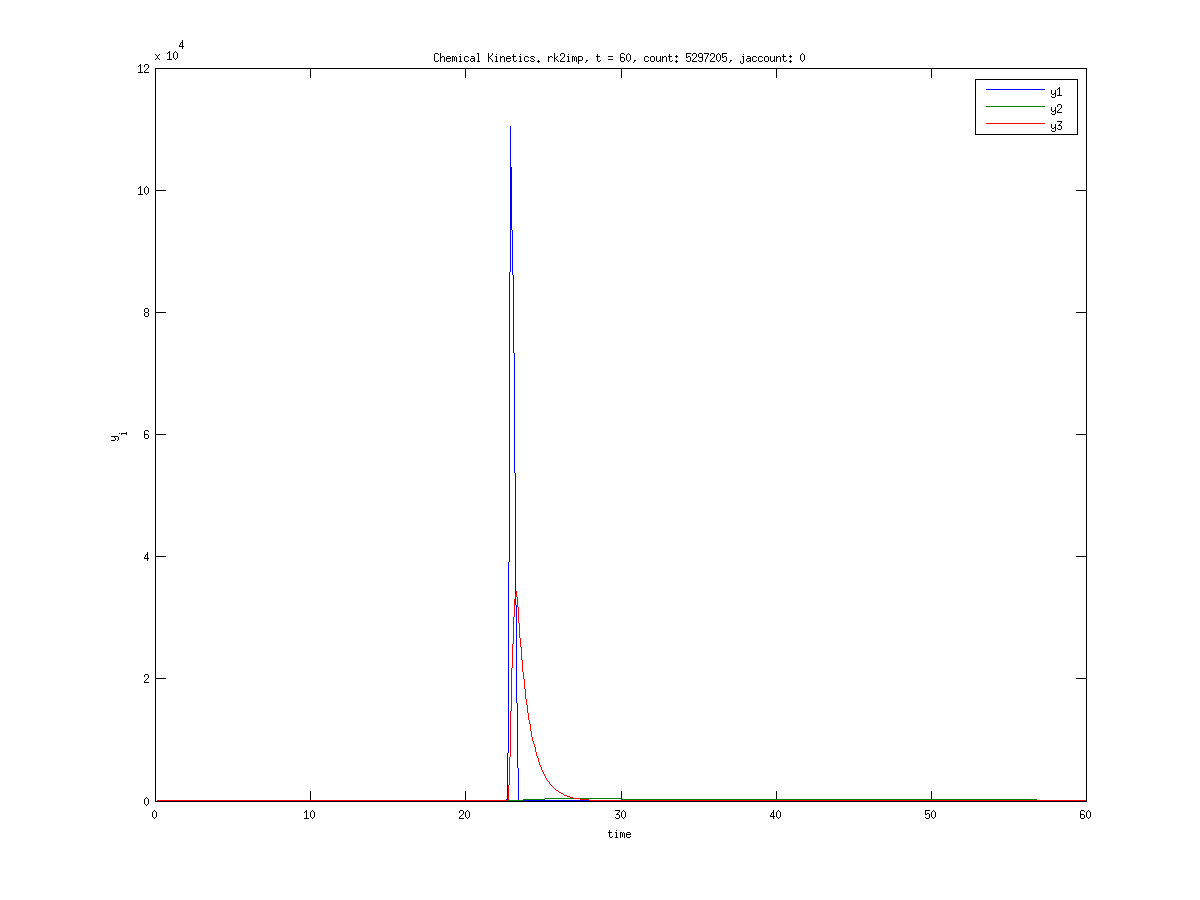
\includegraphics[width=0.8\textwidth]{img/exc2_2_60}
	\caption{Chemical kinetics. Solved using rk2imp integrating from $t=0$ to $t=60$.}
	\label{fig:exc2_2_60}
\end{figure}

\begin{figure}[h!]
	\centering
	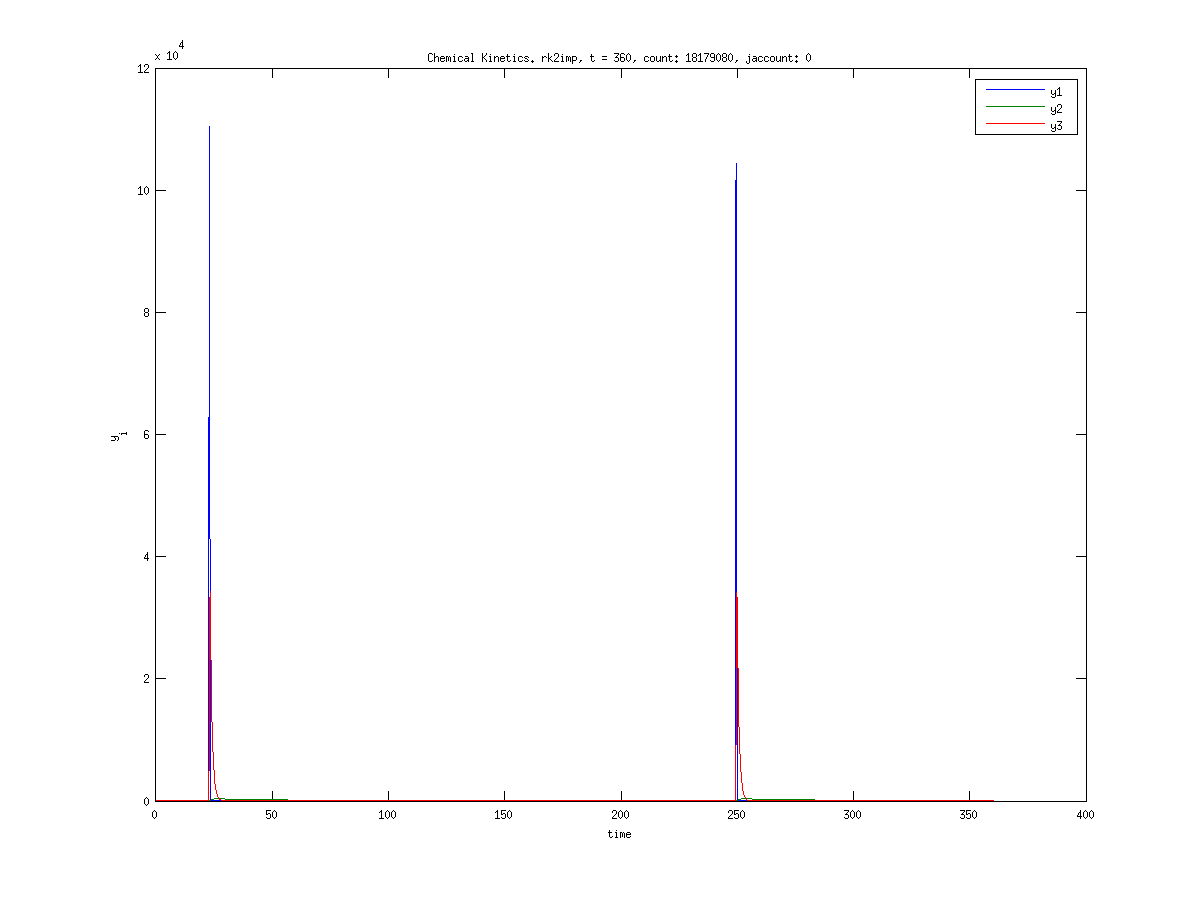
\includegraphics[width=0.8\textwidth]{img/exc2_2_360}
	\caption{Chemical kinetics. Solved using rk2imp integrating from $t=0$ to $t=360$.}
	\label{fig:exc2_2_360}
\end{figure}

\begin{figure}[h!]
	\centering
	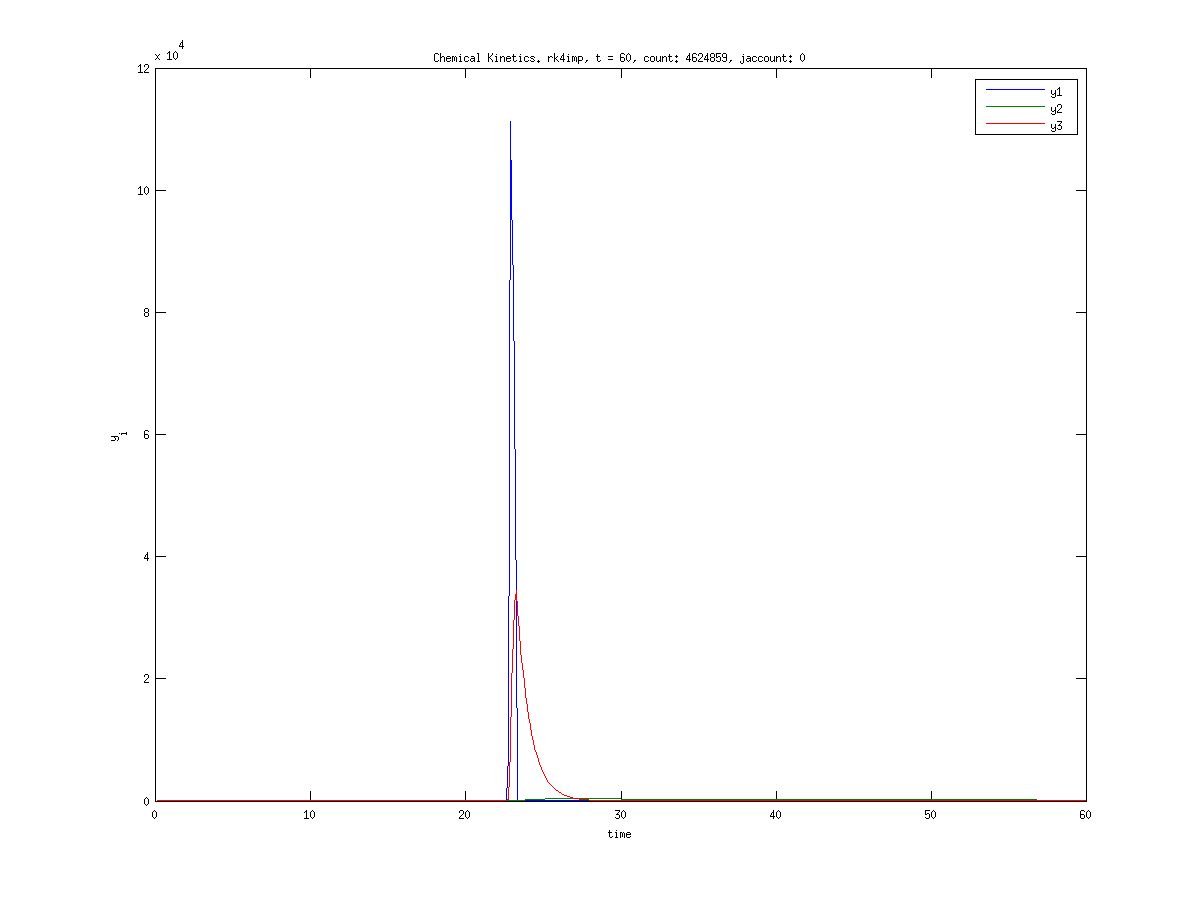
\includegraphics[width=0.8\textwidth]{img/exc2_4_60}
	\caption{Chemical kinetics. Solved using rk4imp integrating from $t=0$ to $t=60$.}
	\label{fig:exc2_4_60}
\end{figure}


\begin{figure}[h!]
	\centering
	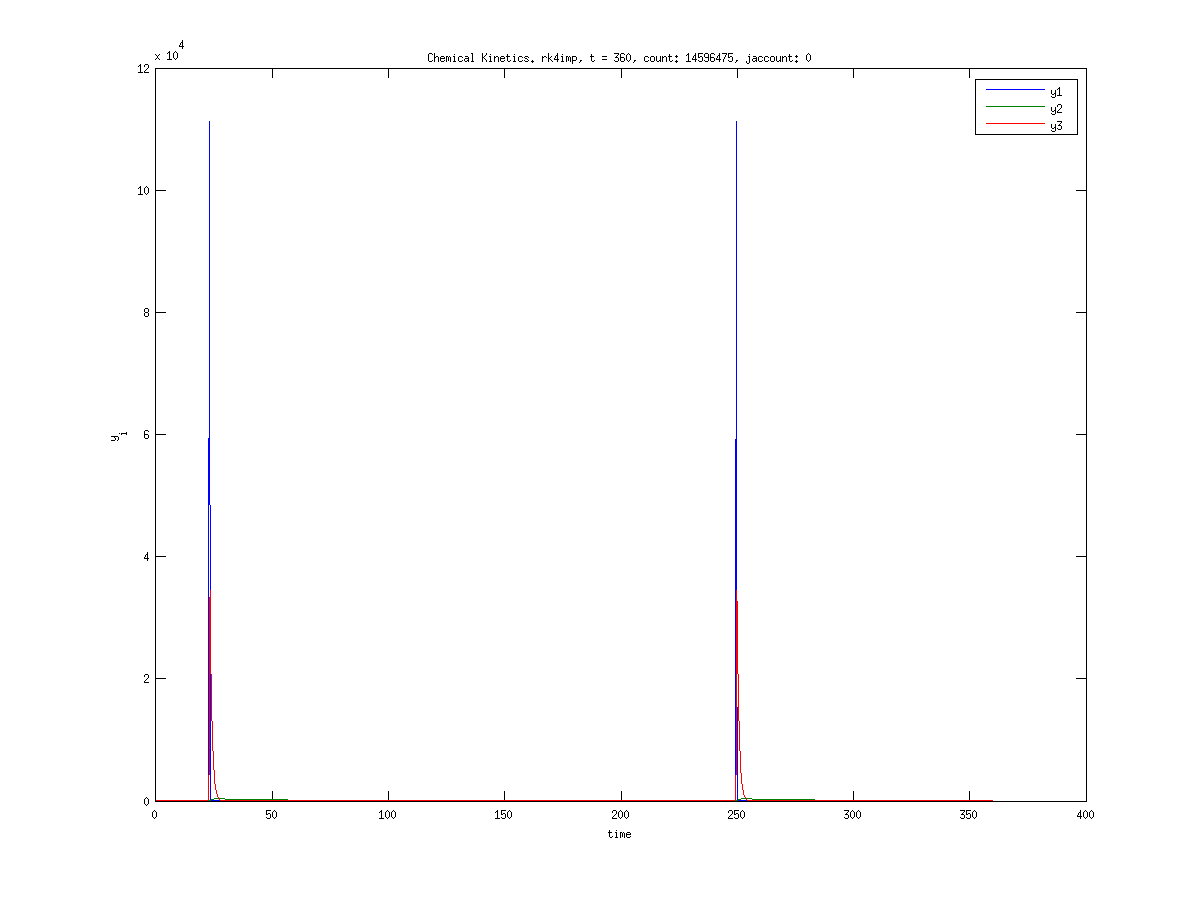
\includegraphics[width=0.8\textwidth]{img/exc2_4_360}
	\caption{Chemical kinetics. Solved using rk4imp integrating from $t=0$ to $t=360$.}
	\label{fig:exc2_4_360}
\end{figure}

The efficiency was about double as fast in the C implementation compared with the matlab implementation. And in the C implementation the rk4imp was better.
The times were: 0.92 seconds from matlab using ode23s; 0.623 seconds in C using rk2imp; 
and 0.419 seconds in C using rk4imp.